
\section{Part IV - State estimation} \label{sec:part4}
%%%% 5.5 
In the earlier problems numerical differentiation have been used to calculate the angular velocities corresponding to the pitch angle, the elevation angle and travel angle. Here an observer to estimate these states was developed instead.

\subsection{Problem 1}
The system \eqref{6a}-\eqref{6c} can be written on the state-space form 
\begin{subequations}
\begin{equation*} 
    \boldsymbol{\dot{x} = Ax + Bu}
\end{equation*}
\begin{equation*}
    \boldsymbol{y = Cx}
\end{equation*}
\end{subequations}
where \textbf{A}, \textbf{B} and \textbf{C} are matrices, and the states are vectors. This was found to be
\[
\begin{bmatrix}
    \dot{\tilde p} \\
    \ddot{\tilde{p}}\\
    \dot{\tilde{e}}\\
    \ddot{\tilde e}\\
    \dot{\tilde{\lambda}}\\
    \ddot{\tilde{\lambda}}
\end{bmatrix}
=
\begin{bmatrix}
    0 & 1  & 0 & 0 & 0 & 0\\
    0 & 0  & 0 & 0 & 0 & 0\\
    0 & 0  & 0 & 1 & 0 & 0\\
    0 & 0  & 0 & 0 & 0 & 0\\
    0 & 0  & 0 & 0 & 0 & 1\\
    K_3 & 0  & 0 & 0 & 0 & 0\\
\end{bmatrix}
\begin{bmatrix}
    \tilde p \\
    \dot{\tilde{p}}\\
    \tilde{e}\\
    \dot{\tilde e}\\
    \tilde{\lambda}\\
    \dot{\tilde{\lambda}}
 \end{bmatrix}
 + 
 \begin{bmatrix}
    0 & 0 \\
    0 & K_1 \\
    0 & 0 \\ 
    K_2 & 0 \\
    0 & 0\\ 
    0 & 0
\end{bmatrix}
\begin{bmatrix}
    \tilde{V_s}\\
    \tilde{V_d}\\ 
\end{bmatrix}
\]
\[
    \begin{bmatrix}
    \tilde{p}\\
    \dot{\tilde{e}}\\
    \tilde{\lambda}
    \end{bmatrix}
=
    \begin{bmatrix}
    1 & 0 & 0 & 0 & 0 & 0\\
    0 & 0 & 1 & 0 & 0 & 0\\
    0 & 0 & 0 & 0 & 1 & 0\\
    \end{bmatrix}
 \begin{bmatrix}
    \tilde p \\
    \dot{\tilde{p}}\\
    \tilde{e}\\
    \dot{\tilde e}\\
    \tilde{\lambda}\\
    \dot{\tilde{\lambda}}
 \end{bmatrix}
\]

\subsection{Problem 2}
Here the task was to examine the observability of the system and create a linear observer for the system. 
To calculate the observability matrix,the MATLAB function obsv(\textbf{A},\textbf{C}) was used. This function calculates the observability matrix of the form 
    \begin{equation}
        \textbf{O} = \begin{bmatrix}
            \boldsymbol{C}\\
            \boldsymbol{AC}\\
             .\\
             .\\
         \boldsymbol{A^{n-1}C}
    \end{bmatrix}
    \end{equation}\label{eq:obsv}
The matrix \textbf{A} has six dimensions, so $n = 6$. By examination of the resulting matrix, the column rank equaled six. From Theorem 6.01 in \cite{syllabus}, this means the matrix has full column rank and therefore the system is observable. 
\newline
Since the system is observable, it was also possible to create the linear observer on the form 
    \begin{equation}\label{eq:state-estimator}
        \boldsymbol{\dot{\hat{x}} = A\hat{x} + Bu + L(y-C\hat{x})}\\
    \end{equation}
with \textbf{L} as the gain observer matrix. The goal for the observer is to estimate the internal state, That $\hat{x} \rightarrow x$, so the error, $e = x - \hat{x}$, approaches zero. This gives the following
    \begin{equation*}
        \boldsymbol{\dot{e} = \dot{x} - \dot{\hat{x}}} = \boldsymbol{Ax - Bu - [A\hat{x} + Bu + L(y-C\hat{x})]}
    \end{equation*}
    \begin{equation}
        \boldsymbol{\dot{e} = (A - LC)e}
    \end{equation}
Hence, its apparent that the dimensions of \textbf{L} are 6x3. To compute \textbf{L} the poles of the system had to be computed first. 
\newline
\newline
The placement of the closed-loop observer poles have an influence on the helicopter since the poles corresponds directly to the eigenvalues of the system through the transfer function. The eigenvalues of the system control the characteristics of the response of the system, meaning that the placement of the poles corresponds to the response of the helicopter.
\newline
\newline
In theory, the poles could be places arbitrarily at whatever desired value, since the system is controllable and observable. This does not mean, however, that the system will work perfect with the chosen value. It was desirable that the poles gave a quick system response, but not too quick, as that may lead to oscillations and a less accurate system. The estimator did give a low-pass filter for the internal state, and filtered the noise for the estimated signal to the system. Another thing to take into account is how big the cut-off frequency the system should have. It should not be to high, as otherwise the measurements could not be trusted, but at the same time they should be low enough to filter out any noise.
\newline
\newline
After many attempts to control the helicopter, it was clear that one could not be so rough with the joystick. This was due to the fact that the helicopter had saturation blocks to keep the input between physical realistic values but the estimator was not saturated in any way. This means that there was a limitation on the motor actuating signal and to much motion in the joystick would not be regulated for as the input would reach saturation. 
\newline
\newline
In \cref{lst:poleplacement}, the different methods for placing poles are demonstrated. For problem 2, after dividing the task into two parts, with and without an integral effect.

\begin{lstlisting}[caption={Matlab code showing different methods for placing poles},label={lst:poleplacement},language=Matlab]
    n = 6;
    poles = zeros(n,1);
    
    %placing poles only on the real axis
    pole = -6;
    for i=1:1:n
        poles(i)=pole;
        pole = pole -2;
    end   
    
    %placing poles in a fan
    theta = pi/15;
    alpha = pi/80;
    r = 50;
    j = sqrt(-1);
    
    for i=1:2:n
        alpha = alpha + theta;
        pole = r * cos(alpha) + j * r * sin(alpha);
        poles(i) = -pole;
        poles(i+1) = -conj(pole);
    end
    
    %placing poles with place function
    L4_2 = place(A4_2', C4_2', poles)';
\end{lstlisting}
The first attempt was to place the poles in a line on the real axis, with varying distance between the poles. Since there were no imaginary parts, the system should be overdamped with no oscillations. But, the result was that the system oscillated to varying degree for all values on the real axis. From the code in \cref{lst:poleplacement}  the poles was placed from -6 to -16 along the real axis as seen in \cref{p4p2nointP6}. The closer the poles were to the origin, the slower the system were and with lower cut-off frequency. Further away the system was faster but with more noise and higher frequency in the oscillations. 

\begin{figure}[H]
\graphicspath{ {Part4_pictures/}}
\begin{subfigure}{0.5\textwidth}
    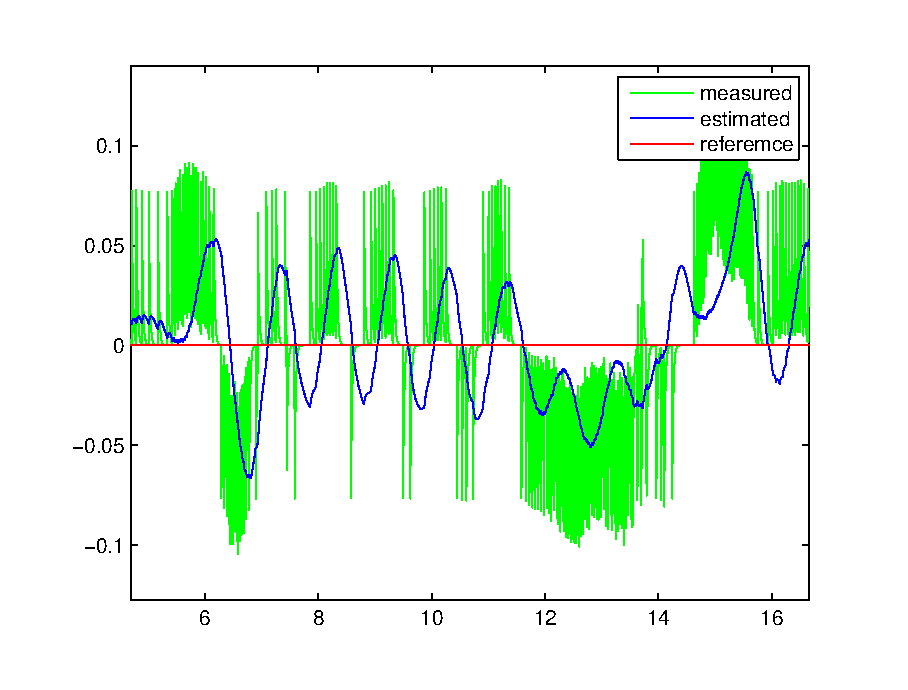
\includegraphics[width=0.9\linewidth]{Part4_pictures/p4p2_noint/riktig_Q/elevationRate_PDreg_P3.eps} 
    \caption{Elevation rate}
    \label{fig:p4p2nointP6e}
\end{subfigure}
\begin{subfigure}{0.5\textwidth}
    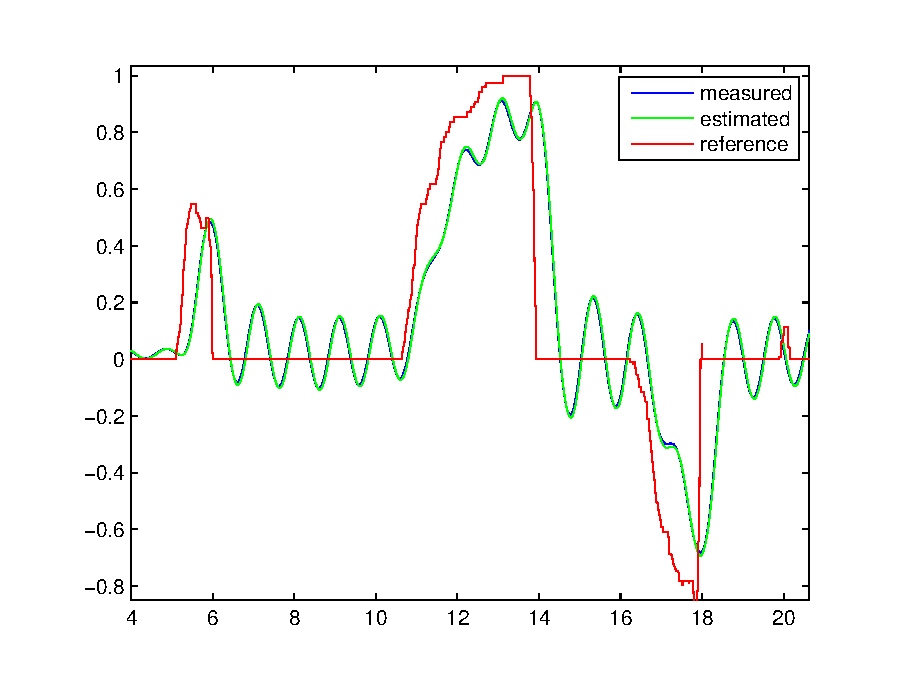
\includegraphics[width=0.9\linewidth]{Part4_pictures/p4p2_noint/riktig_Q/pitch_PDreg_P3.eps}
    \caption{Pitch angle}
    \label{fig:p4p2nointP6p}
\end{subfigure}
\caption{With only real poles and no integral effect, Q = [150 10 250] }
\label{p4p2nointP6}
\end{figure}
The next attempt was placing the poles in a fan formation. The distance between the imaginary and real parts influences how much the system oscillates, in addition to making the system slower or faster. The transient response was fast but it needed tuning to not oscillate as much as with the poles limited the real axis. Making $r = 50$, with $\alpha = \frac{\pi}{50}$ and $\theta = \frac{\pi}{50}$, the response was somewhat slow with a good pitch, but still a little oscillation. 
\newline\newline
An r close to the origin gave a fast response but more oscillation and a poor elevation rate as in \cref{p4p2nointP4}. With r this close to the origin, r being 5, and $\alpha = \frac{\pi}{50}$ and $\theta = \frac{\pi}{15}$ it resulted in oscillations that did not dampen over time. If on the other hand, made r big, towards 100, the helicopter started shaking but the response was still fairly quick. The final value ended with choosing an $r = 50$, with $\alpha$ and $\theta$ equal to $\frac{\pi}{80}$ and $\frac{\pi}{15}$ respectively, as seen in \cref{p4p2nointP1}  This gave a cut-off frequency big enough to have good enough measurements, but still low enough to discard any noise, and poles giving a sufficiently fast transient response.

\begin{figure}[H]
\graphicspath{ {Part4_pictures/}}
\begin{subfigure}{0.5\textwidth}
    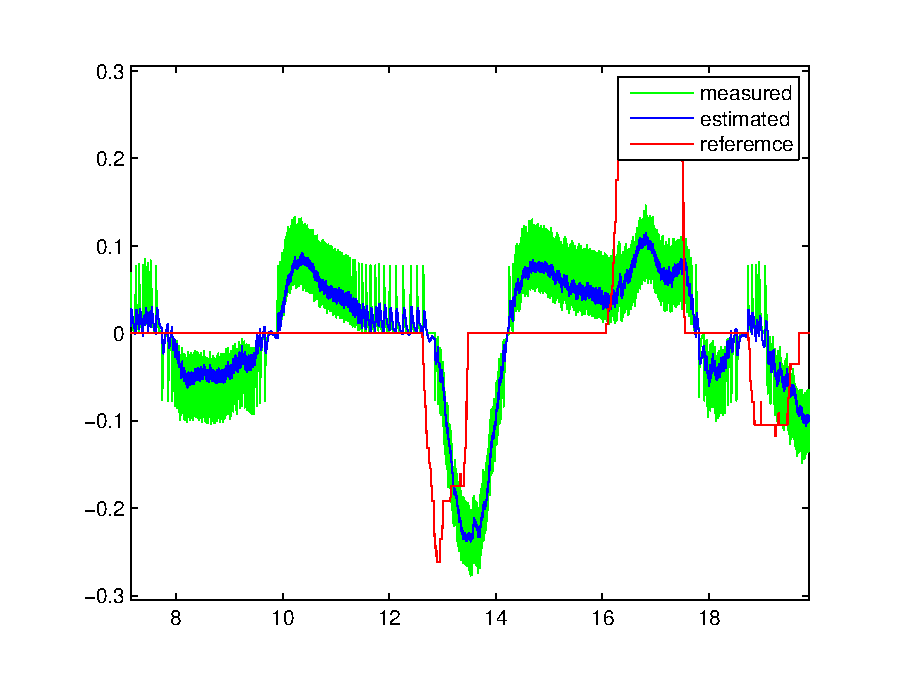
\includegraphics[width=0.9\linewidth]{Part4_pictures/p4p2_noint/riktig_Q/elevationRate_PDreg_P2.eps} 
    \caption{Elevation rate}
    \label{fig:p4p2nointP1e}
\end{subfigure}
\begin{subfigure}{0.5\textwidth}
    \includegraphics[width=0.9\linewidth]{Part4_pictures/p4p2_noint/riktig_Q/pitch_PDreg_P2.eps}
    \caption{Pitch angle}
    \label{fig:p4p2nointP1p}
\end{subfigure}
\caption{Poles in a fan formation with no integral effect. $\alpha = \frac{\pi}{80}$, $\theta = \frac{\pi}{15}$ and r = 50. Q = [150 10 250]}
\label{p4p2nointP1}
\end{figure}
To calculate the observer gain matrix \textbf{L} by hand is far to much work for such a big matrix, thus the \texttt{place} function in MATLAB was used. This function calculates \textbf{L} based on the matrices \textbf{A} and \textbf{C} and pole vector, giving the following matrix:
\[
    \textbf{L} = 10^3 \begin{bmatrix*}[r]
        0.0976 & 0.0133 & -0.0176\\
        2.4106 & 0.6228 & -0.9382\\
        -0.0087 & 0.0943 & -0.0005\\
        -0.4178 & 2.3114 & 0.0515\\
        0.0163 & 0.0038 & 0.0946\\
        0.8242 & 0.2965 & 2.3543\\
    \end{bmatrix*}
    = 
    \begin{bmatrix*}[r] 
        97.6 & 13.3 & -17.6\\
        2410.6 & 622.8 & -938.2\\
        -8.7 & 94.3 & -0.5\\
        -417.8 & 2311.4 & 51.5\\
        16.3 & 3.8 & 94.6\\
        824.2 & 296.5 & 2354.3\\
    \end{bmatrix*}
\]
After tuning without an integral effect, the controller was made to be an PID controller. The same approach to tune the controller was used once more. Trying with the same values as without integral effect gave some oscillation in the pitch angle, more than the elevation. In addition the helicopter dropped down after asking it to rise. Shown in \cref{p4p2intP1} in the Appendix. Using only real poles made the helicopter oscillate particularly violent. This is show in \cref{p4p2intP6}. If the change in the joystick was too quick it made the pitch angle way too big so that it would tip over when using the real poles. \Cref{p4p2intP4} shows the system with the tuning where $r = 50$ with $\alpha = \frac{\pi}{100}$ and $\theta = \frac{\pi}{50}$ that gave the best system.

\begin{figure}[H]
\graphicspath{ {Part4_pictures/}}
\begin{subfigure}{0.5\textwidth}
    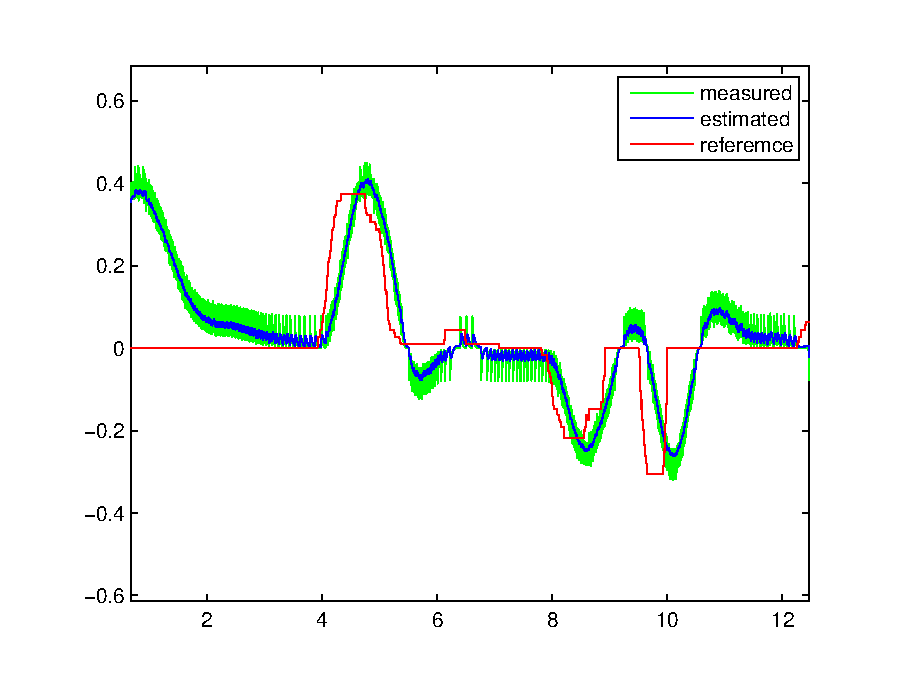
\includegraphics[width=0.9\linewidth]{Part4_pictures/p4p2_int/p4_elevrate_better.eps} 
    \caption{Elevation rate}
    \label{fig:p4p2intP4e}
\end{subfigure}
\begin{subfigure}{0.5\textwidth}
    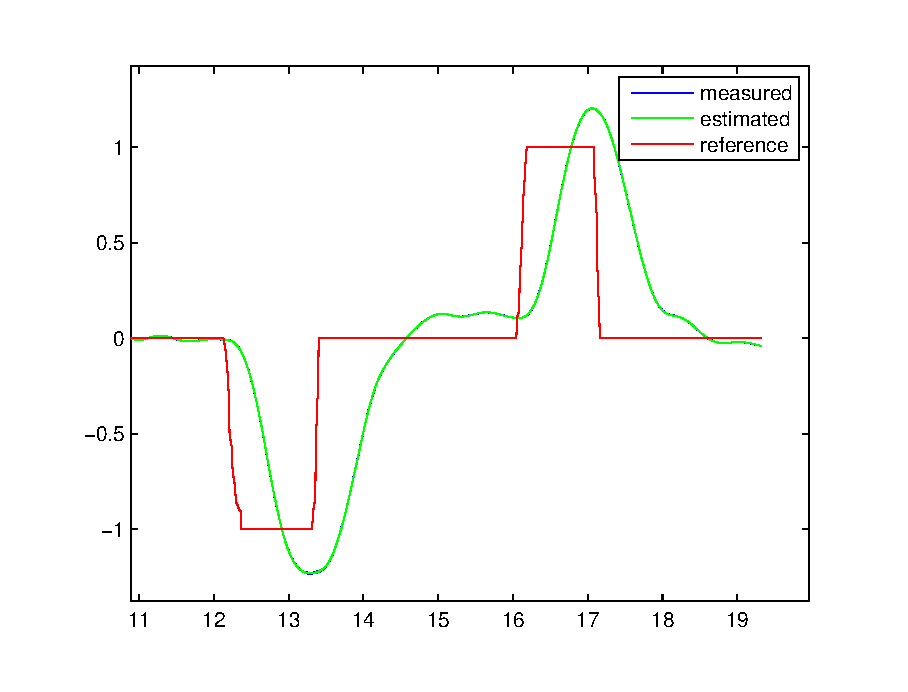
\includegraphics[width=0.9\linewidth]{Part4_pictures/p4p2_int/p4_pitch_better.eps}
    \caption{Pitch angle}
    \label{fig:p4p2intP4p}
\end{subfigure}
\caption{With integral effect. r = 50, $\alpha = \frac{\pi}{100}$ and $\theta = \frac{\pi}{50}$. Q = [50 10 250 50 140]}
\label{p4p2intP4}
\end{figure}

After plotting the estimate, it was possible to see that the estimate was smoother than the measured rate. It almost looks like the estimation was better than the measured value. This is because the estimated value gives the average of the real values of the internal state. The reason why the measured state can be seen as steps in a staircase, was that the measured value takes sample of the real value. In other words, the measured value is a discrete signal, and computers can not take complete analog signals. 

\begin{figure}[H]
    \begin{center}
    \includegraphics[width=0.5\linewidth]{Part4_pictures/estimatorvsmeasured.eps}
    \caption{Observer-signal vs measured -signal }
    \end{center}
\end{figure}
An observation that is worth commenting is something showing up right after starting the helicopter. In \cref{estimation_opservasjon} the estimated signal for the elevation rate drops down and doesn't follow the measured rate at all. This is because the estimator behave like an ordinary differential equation where the true value of the system is the reference for the equation. Like all other differential equation, the response value dampens to the reference. This is what happens when the estimated value bounces from the starting point to its reference which here is the measured value.
\begin{figure}[H]
    \begin{center}
    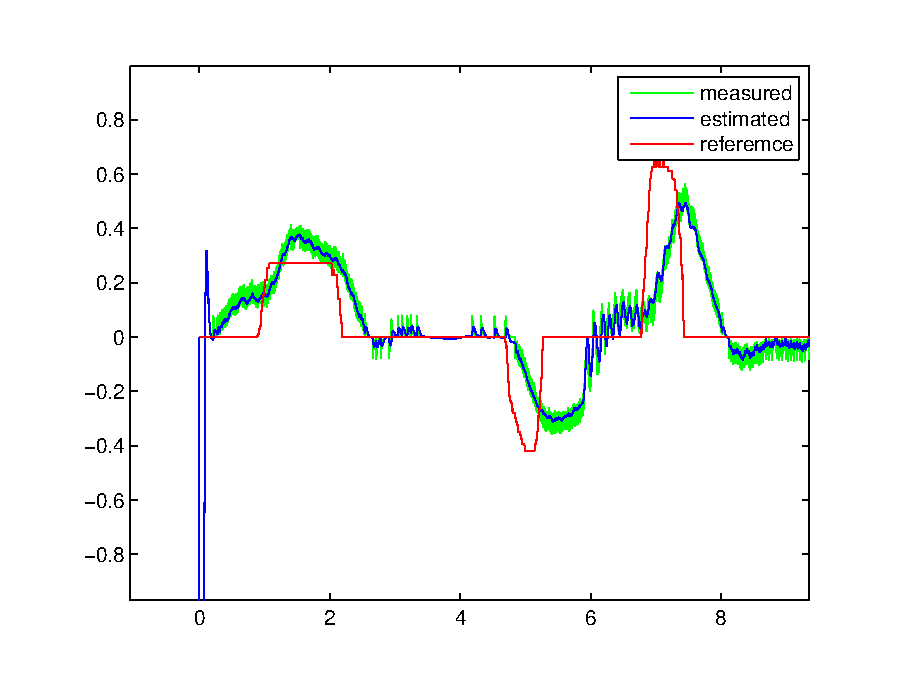
\includegraphics[width=0.5\linewidth]{Part4_pictures/p4p2_noint/p1_elevrate_zoomedin.eps}
    \caption{First second of powering the system}
    \end{center}
    \label{estimation_opservasjon}
\end{figure}

\subsection{Problem 3}
The system can be observable and not observable depending on the choice of the output. If one only measure $\tilde{e}$ and $\tilde{\lambda}$ the system is still observable. The system is not observable if the measurement are from $\tilde{p}$ and $\tilde{e}$. To show this the equation (\ref{eq:obsv}) was calculated in MATLAB, \eqref{lst:p4p3}. For only measuring $\tilde{e}$ and $\tilde{\lambda}$, the \textbf{C} matrix is therefore

\begin{subequations}
\begin{align*}
\textbf{C} = \begin{bmatrix*}
    0 & 0 & 1 & 0 & 0 & 0\\
        0 & 0 & 0 & 0 & 1 &0\\
        \end{bmatrix*}
\end{align*}
\end{subequations}

After the calculation it was easy to see that the rank of the matrix was 6, with full rank. Therefore the system is observable. When the output for the system is $\tilde{p}$ and $\tilde{e}$, the following \textbf{C} is used to calculate the observability matrix.

\begin{subequations}
\begin{align*}
\textbf{C} = \begin{bmatrix*}
        1 & 0 & 0 & 0 & 0 & 0\\
        0 & 0 & 1 & 0 & 0 &0\\
        \end{bmatrix*}
\end{align*}
\end{subequations}
The rank of the observability matrix was found to be four. Hence, the system does not have full rank and is not observable. 
\newline\newline
The task of making a linear observer for $\tilde{e}$ and $\tilde{\lambda}$ was done with the same approach as in 4.2. The dimensions of the \textbf{C} matrix changed, changing the dimensions of \textbf{L} to 6x2. Controlling the helicopter with this linear observer turned out to be very difficult, which was expected as the observer now only has two inputs and does not take the pitch in consideration. As seen in \cref{p4p3comp}, the estimated value for pitch was out of control and made regulation difficult. The poles were first put in a shape of a fan again, but the response was very oscillating and the helicopter was impossible to control. Real poles was now tried, and they were placed close to the origin to get a overdamped system. This would also make the system slower and hopefully it could be possible to somewhat control the helicopter. A happy accident made a pole supposed to be -0.3 to -30 and gave a response where the helicopter didn't crash and behaved somewhat normal. The best response was found with poles = (-0.25,-0.15, -0.2,-0.05, -0.75,-30).

\begin{figure}[H]
\graphicspath{ {Part4_pictures/}}
\begin{subfigure}{0.5\textwidth}
    \includegraphics[width=0.9\linewidth]{Part4_pictures/p4p3/estimate_comp_measured_elevation.eps} 
    \caption{Elevation angle}
\end{subfigure}
\begin{subfigure}{0.5\textwidth}
    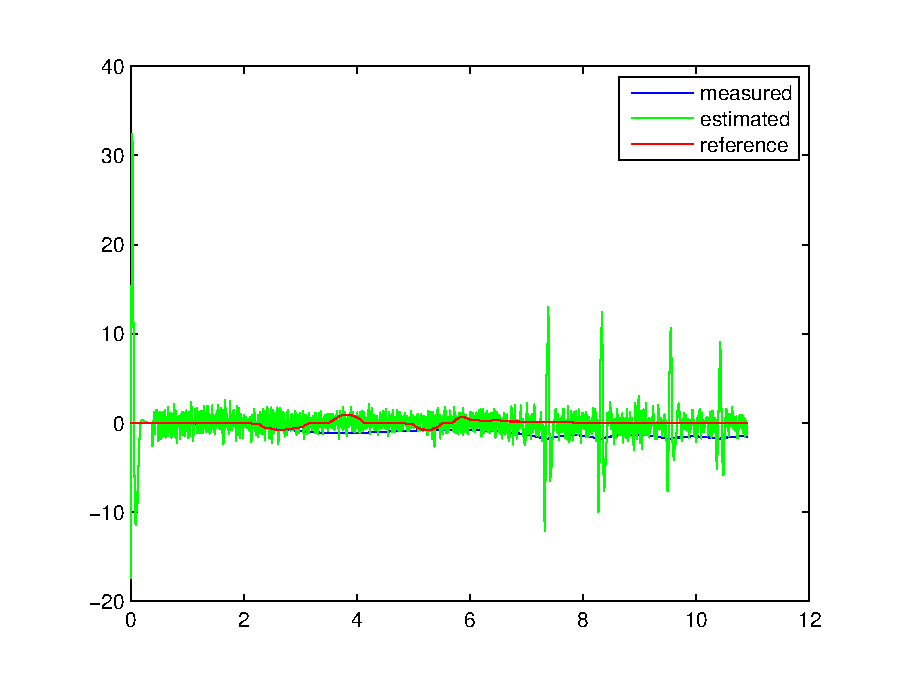
\includegraphics[width=0.9\linewidth]{Part4_pictures/p4p3/estimate_comp_measured_pitch.eps}
    \caption{Pitch}
\end{subfigure}
\caption{Graph to show different behavior of the estimated values with the implemented observer}
\label{p4p3comp}
\end{figure}

To say something about what makes a state estimator poor, it is fitting to start the discussion with the definition of observability. The definition of observability is that a system is observable for any unknown state if for a finite time interval the input and output are sufficient to determine a unique initial state \cite{syllabus}. If the systems output were selected to be $\boldsymbol{y} = [\tilde{e}, \tilde{\lambda}]^T$, then there are enough information to calculate the internal state. For calculating the initial state, information about the initial condition and the input are needed. If all that information for all internal states exists, then every internal state can be estimated and the system is observable. From equation (\ref{6a}-\ref{6c}), it was easy to observe that if not equation (\ref{6c}) was used, then there was no information about the initial condition for the pitch angle $\tilde{p}$. This means the the internal state pitch angle can not be estimated, and the the system is not observable. 